\section{Justificativa}

Apesar do maior interesse recente em SBRS, há questões no tema que carecem de
 pesquisa. A maioria dos trabalhos associados apresenta uma nova arquitetura ou
 um novo modelo de aprendizado de máquina que supera o estado da arte a partir
 de um \textit{dataset} público, por mais que existam aplicações em que uma
 variedade de modelos de base de comparação superam modelos mais arrojados.

 Algumas das oportunidades de pesquisa em SBRS são \cite{rec_sys_handbook_2022}:
 \begin{inparaenum}[(1)]
     \item a integração com as preferências de longo prazo do usuário, em que
     trabalhos publicados sob a temática \textit{session-aware} são minoria;
     \item a inclusão dos metadados associados aos itens;
     \item a maior variedade de domínios -- por exemplo: notícias, varejo,
     música -- dos problemas representados pelos \textit{datasets}; e
     \item a inclusão do contexto atual do usuário -- região, clima, etc. --
     durante a existência de determinada sessão\end{inparaenum}.
     
Por sua vez, o conteúdo do aplicativo Indaband é publicado pelos
usuários, sendo interesse da plataforma oferecer as ferramentas e soluções para
que os usuários publiquem com qualidade suas sessões.
\vspace{0.2cm}
\begin{figure}[ht]
    \centering
    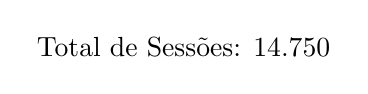
\begin{tikzpicture}
    \pie[ sum=auto, radius=1.4, color={blue!70, orange!70}, after number=\%,
      explode={0, 0.1}, text={}, pos={0,-1}, ]{ 41.3/Publicadas, 58.7/Não
      Publicadas } \node[align=center] at (0,-3) {Total de Sessões: 14.750};
    \end{tikzpicture}
    \hspace{1cm} 
    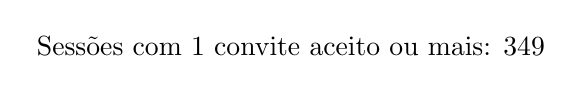
\begin{tikzpicture}
    \pie[ sum=auto, radius=0.8, color={blue!70, orange!70}, after number=\%,
      explode={0, 0.1}, text=legend, pos={0,-1}, ]{ 48.4/Publicadas, 51.6/Não
      Publicadas } \node[align=center] at (0,-3) {Sessões com 1 convite aceito
      ou mais: 349};
    \end{tikzpicture}
    \caption{Sessões e convites enviados. 01/01/2023 a 13/08/2023. Sessões com convites aceitos têm maior taxa de publicação se comparadas ao conjunto completo.}
    \end{figure}
    \vspace{0.2cm}

Sob a perspectiva comercial, o seguinte indício sustenta que um SBRS pode
aumentar a taxa de sessões publicadas pelos usuários do Indaband: apenas 1.146
(7,77\%) das 14.750 sessões criadas em 2023 até 13 de agosto contém no mínimo um
convite emitido. Afunilando ainda mais, a análise das taxas de publicação indica
que as sessões com ao menos um convite aceito, que são apenas 349 (2,37\%) das
14.750 sessões totais criadas, tem maior taxa de publicação se comparada ao
conjunto de todas as sessões. Portanto, uma forma simples de aumentar a taxa de
publicação geral da plataforma é permitir que o conjunto de sessões com
convidados seja maior, o que pode ser incentivado ao integrar um SBRS ao
aplicativo.

Sob a perspectiva de viabilidade técnica, de todas as 14.750 sessões criadas
em 2023 até 13 de agosto, 6.857 (46,5\%) foram criadas com ao menos dois
usuários que gravaram as faixas existentes. Isso é possível a partir da
funcionalidade de \textit{fork}, que permite a cópia de uma sessão publicada
com suas faixas originais. Basta um novo usuário versionar uma sessão com uma
única faixa de outro usuário para que exista associações entre esse novo
usuário e os demais que o segundo usuário já tenha colaborado.

\vspace{0.2cm}
\begin{figure}[H]
      \centering
      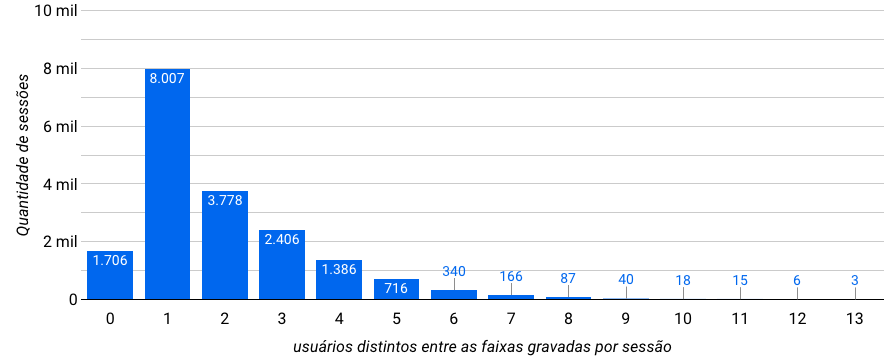
\includegraphics[width=1\textwidth]{chapters/chap01/images/plots/users.png}\vfill
      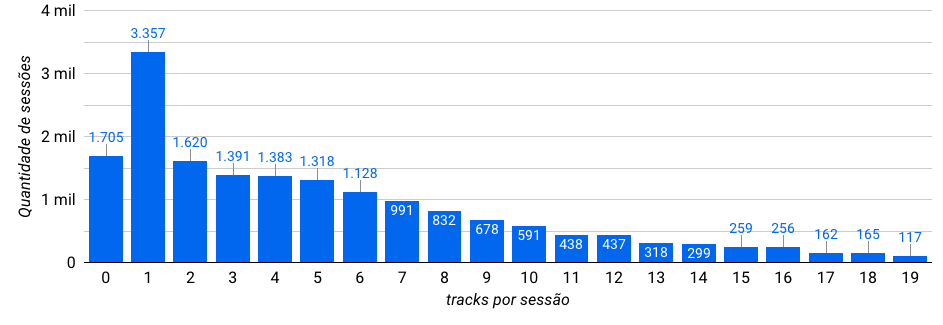
\includegraphics[width=1\textwidth]{chapters/chap01/images/plots/tracks.png}
      \caption{Dados de sessões em 2023 até o presente momento. A quantidade de \textit{tracks}
       e usuários por sessão sustenta a viabilidade técnica de um modelo de
       aprendizado de máquina para a recomendação de convites.}
      \label{fig:combined}
  \end{figure}
\vspace{0.2cm}
